\chapter{ Методи, средства и методологии за изработване на бойни роботи}

%================================================================================
% ЗАДВИЖВАНЕ

\section{Основни методи и технологии за задвижване на бойни роботи}
\label{sec:motion-types}

Бойните роботи традиционно могат да се задвижват по три начина чрез вериги, колела или механични крака. Има и други начини, но те не са ефективни в битка.
Роботите, задвижвани с танкови вериги, имат отлично сцепление със земята и вървят много стабилно, но имат много недостатъци. Поради голямата площ на триене при завъртане те изразходват значително количество енергия. Освен това и самото движение се извършва сравнително бавно, което позволява на опонента да заобиколи робота и да го удари в гръб. Боен робот, задвижван от верига, може да се види на \cref{fig:using-treads}.

\begin{figure}[H]
    \centering
    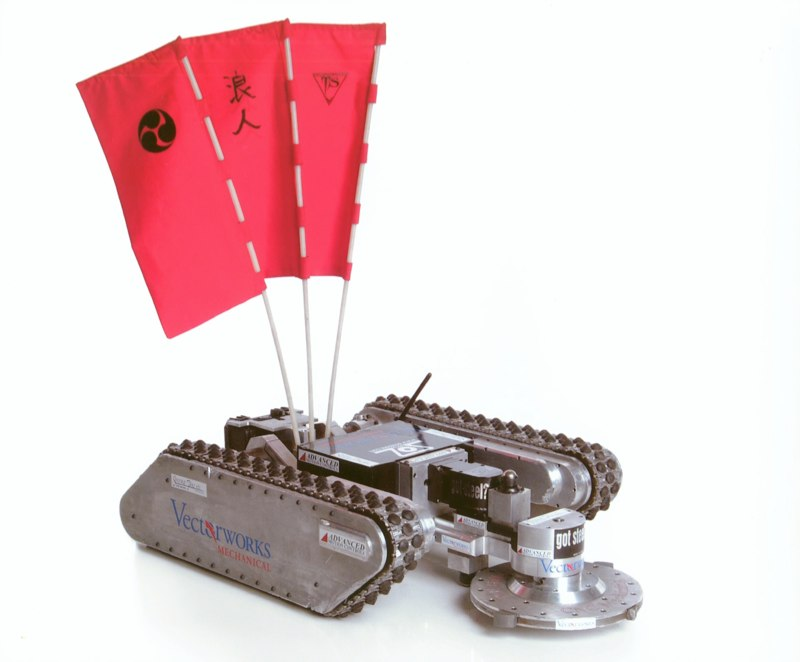
\includegraphics[width=0.5\linewidth]{images/using-treads.jpg}
    
    \caption{Боен робот, задвижван от вериги}
    \label{fig:using-treads} 
\end{figure}

Механичните крака имат също много недостатъци. Някои от които са, че са много сложни за конструкция и контрол. Друг техен недостатък е, че те не са достатъчно здрави по време на битка, особено срещу посичащите спинер роботи. Повече за този тип бойни роботи може да се прочете в \cref{sec:robot-types}. Трета слабост е, че центъра на тежестта на роботи с такава система за задвижване е много високо над земята, което ги прави уязвими срещу атаки, целящи преобръщане. Батълбот, използващ механични крака може да бъде видян на \cref{fig:using-legs}.

\begin{figure}[H]
    \centering
    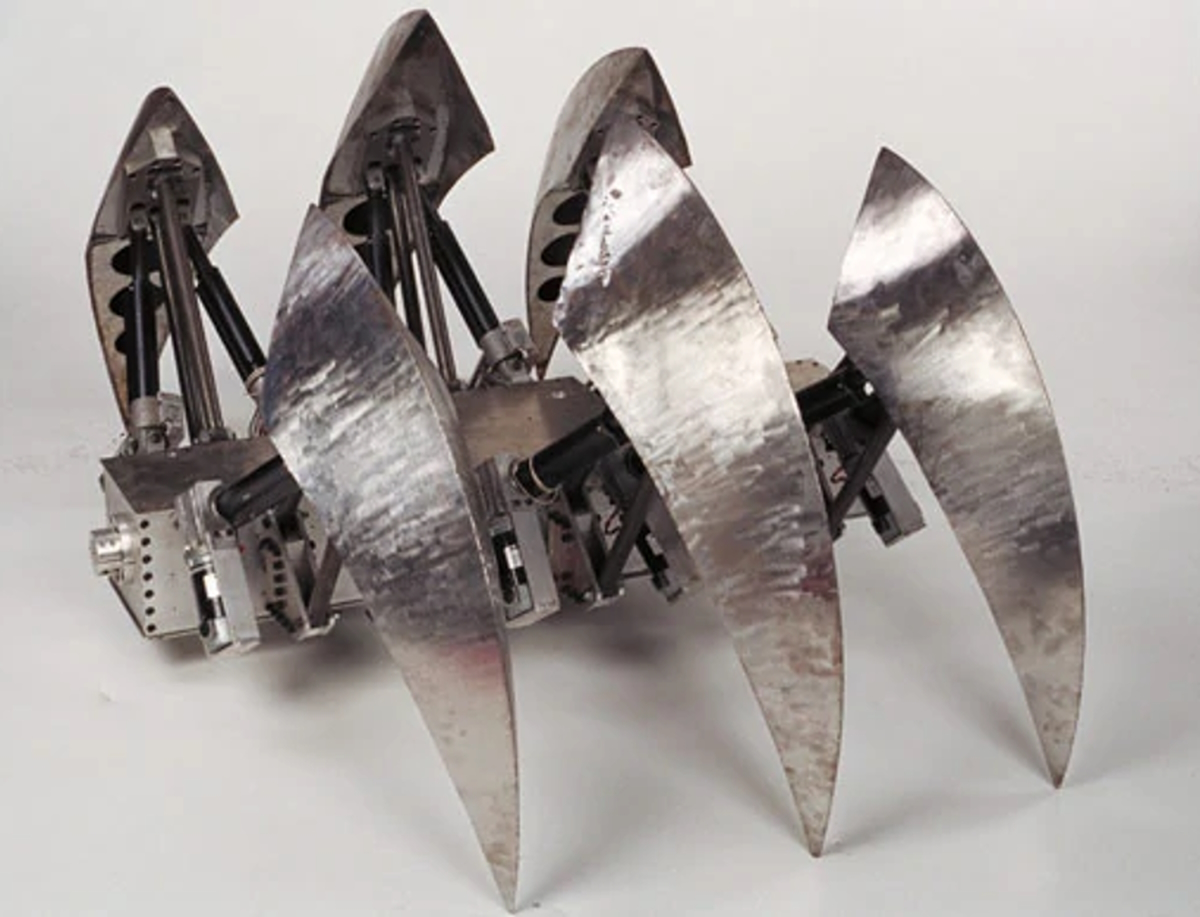
\includegraphics[width=0.6\linewidth]{images/using-legs.jpg}

    \caption{Боен робот, задвижван от механични крака}
    \label{fig:using-legs} 
\end{figure}

Поради гореспоменатите причини, най-често бойните роботи се задвижват чрез колела. Разпространени са два начина на управление на задвижването на моторни средства с колела – Акерман управление и диференциално управление. Акерман управлението е възприето от повечето моторни-превозни средства. При него един голям мотор задвижва колелата и един по-малък отговаря за тяхното завъртане. То е ефективно при движение в права линия, но когато трябва да се завие се изискват определени маневри. Диференциалното управление е много по-често срещано в роботиката. При него лявата и дясната страна на робота се задвижват напълно индивидуално. Недостатъкът на този метод е фактът, че за да се движи моторното средство в права линия двете половини требва да имат еднаква скорост, което е трудно за постигане. Голямото преимущество обаче е, че завиването става значително по-бързо.

Освен по начин на управление на задвижването роботите придвижващи се с колела се различават помежду си и чрез броя на задвижваните колела. При такива с две задвижващи колела и диференциално управление на задвижването, завиването се случва със сравнително ниски загуби на енергия. Проблемът е, че с две опорни точки, роботът най-вероятно ще има нужда от поне още една такава. Той се решава чрез добавянето на ball transfer units.


%================================================================================
% КОМУНИКАЦИЯ

\section{Основни методи и технологии за дистанционно управление на бойни роботи}

Съгласно официалните изисквания за работа към бойните роботи, те трябва да бъдат контролирани безжично дистанционно. За целта могат да се използват много технологии за безжична комуникация, като едни от най–популярните са Wi-Fi, Bluetooth и nRF24L01.

Wi-Fi позволява много висока скорост на предаване на информацията, но има много недостатъци. Един от тях е, че има много високо потребление на енергия. Друг е, че не може директно да се предава информация от едно устройство на друго безжично, а първо трябва тази информация да се подаде на маршрутизатор и след това той да я изпрати до устройството получател. Отделно по време на боевете се очаква да има голяма публика и безплатен Wi-Fi което предполага, че каналите, които се използват за тази технология ще бъдат претоварени и съответно ще има по-лоша свързаност. 

Bluetooth технологията осигурява средна скорост на предаване на информация, на цената на средно ниво на консумация на енергия. Недостатъкът е, че за да могат две устройства да се свържат и да общуват безжично и двете трябва предварително да се сдвоят, което е непрактично за системи, които не включват компютри или телефони.

Модулът nRF24L01 позволява безжична радиочестотна комуникация с други такива модули. От трите технологии за безжична комуникация този модул предлага тази с най-ниско потребление на енергия. За разлика от Wi-Fi, nRF24L01 може да се комуникира с друго устройство директно, без необходимостта от маршрутизатор. Предимството му пред Bluetooth е, че не е необходимо предварително двете устройства да се сдвояват.

\begin{table}[H]
    \centering
    \begin{tabular}{| m{4cm} | m{3,5cm} | m{3,5cm} | m{3,5cm} |}
        \hline
        & Wi-fi & Bluetooth & nRF24L01+ \\
        \hline
        Скорост &  Висока & Средно & Средна \\
        \hline
        Обхват & 10ки метри & 10 метра & 10-150 метра \\
        \hline
        Енергийна консумация & Висока & Средна & Ниска\\
        \hline
    \end{tabular}
    \caption{Сравнителна таблица за безжични технологии}
    \label{table:wireless}
\end{table}


%================================================================================
% БРОНЯ

\section{Основни методи за защита на бойни роботи}

За защита на бойните роботи винаги се монтира броня около неговата структура. Видовете броня са: традиционна, аблативна и реактивна.

Традиционната броня е изработена от много здрави и твърди материали, които се стремят да абсорбират и предадат енергията на удара без да се повреждат. Високата твърдост и здравина на този вид защита често се използва за чупене или изтъпяване на остриетата на вражеските оръжия и запазване целостта на робота при удари. Благодарение на здравината си тази броня по-рядко трябва да се сменя след битки, но нейният недостатък е, че при удар енергията на сблъсъка се предава до елементите вътре в робота, което може да доведе до тяхното повреждане.

Аблативната защита, от друга страна е проектирана да предпазва от щети робота, като самата тя бива повреждана чрез процеса аблация. Това е процеса на премахване на материал от повърхността на обект посредством изпарение или стружко отделяне. Материалите, от които е изградена са също твърди и здрави, но за разлика от традиционната броня имат по-ниска твърдост. Поради това тяхно свойство, когато тези брони трябва да предпазват от силни удари, вътрешните елементи биват изложени на риск. Материали като дървото са много ефикасни представители на този вид елементи, но друг техен недостатък е, че сблъсъците водят до много визуални следи, което често носи допълнителни точки на опонента за щети.

Третия вид броня е реактивната. По време на удар тя реагира по някакъв начин, за да предотврати щети. Има различни видове реактивна броня и всяка има свой предимства и недостатъци. Пример за такъв вид защита е пласт гума между два пласта метал. Предимството й е, че в случай на удар, пластът гума би абсорбирал енергията на удара. Този вид броня не е ефективна в боевете с роботи, поради причината, че много бързо бива повреждана и спира да пази.

%================================================================================
% ВИДОВЕ РОБОТИ

\section{Видове съществуващи бойни роботи}
\label{sec:robot-types}

Съществуват много различни видове батълботи. Основно изискване към всеки от тях е да имат поне едно оръжие, чрез което да могат да повредят опонента. В зависимост от своето оръжие роботите се разделят на 14 типа: „rammer“, „wedge“, „lifter“, „flipper“, „spearbots“, „horizontal spinner“, „sawbot“, „vertical spinner“, „drumbot“, „hammerbot“, „clamper“, „crusher“, „flamethrower“ и „multibot“. Има и други видове роботи, но те почти винаги могат да бъдат категоризирани в един от гореспоменатите видове. За ефективността на бойния робот в битка има голямо значение какво оръжие е избрано. Примерно със своите огромни дискове нанасящи разрушителни удари роботите с оръжие „vertical spinner“ са много ефективни срещу голяма част от роботите. Те имат обаче един фатален недостатък, който се изразява в това, че поради голямата скорост на въртене на съответното оръжие генерират жироскопичен ефект, който намалява осезателно скоростта им на движение, което ги прави уязвими към удари отзад. С времето в роботските боеве категориите „flipper“, „horizontal spinner“, „vertical spinner“, „drumbot“, „hammerbot“ и „clamper“ са се откроили като по-ефективни в сравнение с останалите.
